\newif\ifcomments
%\commentsfalse
\commentstrue

\newif\ifclaude
\claudefalse

\documentclass[letterpaper,12pt,usenames,dvipsnames]{article}

\frenchspacing

%\usepackage[margin=1in, includefoot]{geometry}

\usepackage{amsmath}
\usepackage{amssymb}
\usepackage{amsthm}
\usepackage{changepage}
\usepackage{setspace}
\usepackage{mathpazo}
\usepackage{float}
\usepackage{pdflscape}
\usepackage{siunitx}
\usepackage[margin=1in]{geometry}
\usepackage[colorlinks=true, allcolors=black]{hyperref}
\usepackage{amsfonts}
\usepackage{booktabs}
\usepackage{caption}
\usepackage{subcaption}
\usepackage{tabularray}
\UseTblrLibrary{booktabs}
\usepackage[longnamesfirst]{natbib}
\usepackage{tikz}

% Paper tables are generated from aggregate pipeline outputs under output/paper/.
% A missing file renders as a labeled placeholder so the draft still compiles.
\newcommand{\paperdir}{../output/paper}
\newcommand{\inputpaper}[1]{%
	\IfFileExists{\paperdir/#1}{\input{\paperdir/#1}}{%
		\fbox{\parbox{0.9\linewidth}{\centering\small
			Generated table not yet available: \texttt{output/paper/\detokenize{#1}}}}}%
}

\newcommand{\sumn}{\sum_{i=1}^{n}}
\newcommand{\sumt}{\sum_{t=0}^\infty}
\newcommand{\sums}{\sum_{t=0}^\infty \sum_{s^t}}
\newcommand{\sumj}{\sum_{j=-\infty}^\infty}
\newcommand{\fsum}{\frac{1}{n} \sum_{i=1}^n}
\newcommand{\prodn}{\prod_{i=1}^{n}}
\newcommand{\intf}{\int_{-\infty}^{\infty}}
\newcommand{\intz}{\int_0^\infty}
\newcommand{\limf}{\lim_{n\to \infty}}
\newcommand{\I}{\mathbb{I}}
\newcommand{\N}{\mathbb{N}}
\newcommand{\R}{\mathbb{R}}
\newcommand{\E}{\mathbb{E}}
%\newcommand{\E}{E}
\newcommand{\Z}{\mathbb{Z}}
\newcommand{\C}{\mathbb{C}}
\newcommand{\M}{\mathcal{M}}
\newcommand{\bp}{\mathbb{P}}
\newcommand{\F}{\mathcal{F}}
\newcommand{\Cost}{\text{Cost}}
%\newcommand{\pay}{\text{pay}}
\newcommand{\cH}{\mathcal{H}}
\newcommand{\Var}{\text{Var}}
\newcommand{\Cov}{\text{Cov}}
\newcommand{\topr}{\xrightarrow{  p  }}
\newcommand{\tod}{\xrightarrow{  d  }}
\newcommand{\blambda}{\bar{\lambda}}
\newcommand{\htheta}{\hat{\theta}}
\newcommand{\hbeta}{\hat{\beta}}
\newcommand{\hmu}{\hat{\mu}}
\newcommand{\hF}{\hat{F}}
\newcommand{\sss}{\subsubsection*}
\newcommand{\simiid}{\stackrel{\text{iid}}{\sim}}
\newcommand{\eqas}{\stackrel{\text{a.s.}}{=}}
\newcommand{\eps}{\varepsilon}
\newcommand{\re}{\text{Re}}
\newcommand{\im}{\text{Im}}
\newcommand{\cond}{ \; \Bigr| \; }
\newcommand{\maxtil}{ \widetilde{\max} }

\newcommand{\dxdy}[2]{\frac{\partial #1}{\partial #2}}
\newcommand{\ind}[1]{\mathbf{1}_{\{ #1 \} }}
\newcommand{\til}[1]{\tilde{#1}}
\newcommand{\noth}[1]{#1}

\newcommand{\pbrac}[1]{\left( #1 \right)}
\newcommand{\Bigpbrac}[1]{\Bigl( #1 \Bigr)}
\newcommand{\Biggpbrac}[1]{\Biggl( #1 \Biggr)}
\newcommand{\bigpbrac}[1]{\bigl( #1 \bigr)}
\newcommand{\biggpbrac}[1]{\biggl( #1 \biggr)}

\newcommand{\sbrac}[1]{\left[ #1 \right]}
\newcommand{\Bigsbrac}[1]{\Bigl[ #1 \Bigr]}
\newcommand{\Biggsbrac}[1]{\Biggl[ #1 \Biggr]}
\newcommand{\bigsbrac}[1]{\bigl[ #1 \bigr]}
\newcommand{\biggsbrac}[1]{\biggl[ #1 \biggr]}

\newcommand{\cbrac}[1]{\left\{ #1 \right\}}
\newcommand{\Bigcbrac}[1]{\Bigl\{ #1 \Bigr\}}
\newcommand{\biggcbrac}[1]{\biggl\{ #1 \biggr\}}
\newcommand{\bigcbrac}[1]{\bigl\{ #1 \bigr\}}
\newcommand{\Biggcbrac}[1]{\Biggl\{ #1 \Biggr\}}

\newcommand{\pfrac}[2]{\pbrac{\frac{#1}{#2}}}

\newcommand{\undertext}[2]{\underbrace{#1}_{\text{#2}}}

\newcommand{\tblrsection}[2]{\midrule \SetCell[c=#1]{c} \textit{#2} \\ \midrule}
\newcommand{\tablesection}[2]{\midrule \multicolumn{#1}{c}{\textit{#2}} \\ \midrule}

\newcommand{\todo}[1]{\ifcomments{\color{red} [#1]}\fi}

\newcommand{\round}[2]{%
	\qty[round-mode=places, round-precision=#2]{#1}%
}

\allowdisplaybreaks[1]

%\numberwithin{equation}{section}

\theoremstyle{definition}
\newtheorem{thm}{Theorem}
\newtheorem{claim}{Claim}
\newtheorem{prop}[thm]{Proposition}
\newtheorem{defn}{Definition}
\newtheorem{cor}{Corollary}
\newtheorem{ex}{Example}
\newtheorem{exer}{Exercise}
\newtheorem{lem}[thm]{Lemma}
\newtheorem{ob}{Observation}
\newtheorem{fact}{Fact}

\onehalfspacing

\begin{document}

%\ifnotaer
%\small
%\fi
% \footnotesize

%\def\plotdir{C:/Users/Dan/Dropbox/output/frm}
\def\drop{/home/dan/Dropbox}
\IfFileExists{localpaths.tex}{\input{localpaths.tex}}{}

\newenvironment{tablenotes}{\begin{spacing}{1.0} \footnotesize \emph{Note:} }{\end{spacing}}
\newenvironment{figurenotes}{\begin{spacing}{1.0} \footnotesize \emph{Note:} }{\end{spacing}}

\title{Classifying Second Liens in Historical \\ Home Mortgage Disclosure Act Data} 
\author{Daniel L. Greenwald\thanks{Leonard N. Stern School of Business
		Kaufman Management Center, 44 West Fourth Street, New York, NY 10012; Email: \texttt{dlg340@stern.nyu.edu}.}
	}
\date{}

\maketitle

\begin{abstract}
\noindent \todo{TBC}
\end{abstract}

  
%\clearpage
\section{Introduction}

\section{Data}\label{sec:data}


\subsection{Home Mortgage Disclosure Act Data}\label{sec:hmda-data}

Our main data source is the HMDA Loan Application Register (LAR) files for 1990--2016, which contain the near-universe of originated home mortgages in the US. We obtain these files from three sources: \todo{FILL IN SOURCE BY YEAR}.

This dataset includes the loan amount, applicant income, loan type, purchaser type (the type of institution that purchased the loan), the loan outcome (i.e., whether it was originated), and the state and county in which the property resides. Beginning in 2004, these data also include an indicator for whether a loan is a second lien. However, prior to 2004, this field is not available, motivating the estimation below.

For my analysis, I restrict the sample to originated owner-occupied purchase loans, and drop any observations with missing values for loan amount, applicant income, loan type, purchaser type, loan outcome, state, and county. I further restrict the sample to observations that: (i) are located in the 50 states or District of Columbia; (ii) have strictly positive values for applicant income and loan amount, and (iii) have one of the four standard loan types (conventional, FHA, VA, and FSA/RHS) \todo{make sure these acronyms are defined somewhere}. From 2004 on, I also require a non-missing value for second-lien status. These restrictions lead to a final sample of 90.2 million observations from an original pool of 542.4 million observations, with most of the attrition (to 95.5 million) stemming from my restriction to originated owner-occupied purchase loans.

\subsection{County House Price Data}\label{sec:fhfa-data}

While the loan-to-income ratio can be constructed directly from HMDA data, the prevailing value of properties may also be informative for determining the distribution of typical first and second lien sizes in a given area. Since I cannot match transactions with the sales price for that particular property, I instead merge in data on house prices at the county level.

For this house price series, I use two complementary sources. First, I use the all-transactions county house price index from the FHFA \citep{bogin2019local,fhfa2026county}. This source has excellent temporal coverage, and is available for all years of our 1990--2016 sample. However, these price indices are normalized separately by county, and cannot be directly interpreted using a dollar value. To address this, I incorporate the Zillow Home Value Index (ZHVI), obtained from \cite{zillow2026zhvi}. This index is scaled in dollar amounts, corresponding to the median home value in each county, but is not available prior to \todo{FILL}.

Using these series, I create a combined house price index
\begin{align}
	\label{eq:house-price-index}
	\log v_{c,t} = \log v^{FHFA}_{c,t} + \log a_c
\end{align}
where $c$ denotes county, $t$ denotes time, $v^{FHFA}_{c,t}$ is the FHFA house price index, and $a_c$ is a scaling factor designed to convert the FHFA series from a normalized index to dollar levels. These scaling factors are in turn computed as
\begin{equation}
	\log a_c = \frac{1}{T_{max} - T_{min}} \sum_{t=T_{min}}^{T_{max}}
	\pbrac{\log v^{ZHVI}_{c,t} - \log v^{FHFA}_{c,t}},
	\label{eq:county-value}
\end{equation}
where $T_{min}$ and $T_{max}$ are the start and end years of the overlapping sample over which both indices are vailable. Combined, equations \eqref{eq:house-price-index} and \eqref{eq:county-value} ensure that the final series $v_{c,t}$ has the same relative values as in the FHFA series, but has an average log level equal to that of the ZHVI index when both series are available.

\ifclaude

The analysis uses the annual national Home Mortgage Disclosure Act (HMDA) Loan/\allowbreak Application
Register (LAR) files for 1990--2016 \citep{avery2007opportunities}. Each record describes a
mortgage application or purchased loan reported by a covered lender, including the loan amount,
applicant income, loan type, the type of institution that purchased the loan within the
calendar year, and the property's state and county. The field that motivates this paper is lien
status. Following the 2002 amendments to Regulation C, lenders began reporting whether an
originated loan is secured by a first or a subordinate lien with the 2004 data; the field does
not exist in earlier LARs. We therefore treat 2004--2016 as labeled years and 1990--2003 as
unlabeled application years. Provider-specific file layouts are mapped to a single versioned
variable schema before any sample restriction is applied.
\todo{Document the source vintage used for each year (NARA, FFIEC, CFPB) once raw-file
sourcing is final; see data/README.md. State why 2017, the last pre-2018-format year, is
excluded.}

The target population is originated, owner-occupied, home-purchase loans. From the raw LAR we
retain records whose action is an origination, whose purpose is home purchase, and whose
property is owner occupied. We then require (i) a state in the 50 states or the District of
Columbia and a nonmissing county code; (ii) positive, nonmissing applicant income and loan
amount, both of which HMDA reports in thousands of dollars; (iii) one of the four standard loan
types (conventional, FHA, VA, and FSA/RHS); and (iv) a county-value match, described in
Section~\ref{sec:data_predictors}. In labeled years we also require a nonmissing lien status.
Within this sample the reported field takes only the first-lien and subordinate-lien values, so
no further restriction on the label is needed.

Across the 27 years, the origination, purpose, and occupancy restrictions retain 95.45 million
of 542.38 million raw records. Missing or invalid geography removes a further 3.2 percent of
these loans, and missing or invalid income or loan amount removes 2.4 percent, leaving 90.23
million eligible loans before the county-value merge. The merge is nearly complete in the
labeled period: it retains 99.75 percent of eligible 2004--2007 loans and at least 99.47
percent in every year from 2000 onward. Coverage is lower early in the sample---96.42 percent
of eligible loans in 1990---because many low-volume counties lack a scaled county value.
Table~\ref{tab:sample} reports representative years, and Appendix~\ref{app:data} reports the
complete annual attrition.

A final restriction requires finite values of all four predictors, so every model in the paper
scores exactly the same observations. It binds only because of missing purchaser type in three
historical years, removing 700 of 1,664,933 otherwise eligible loans in 1990 (0.042 percent),
195 of 1,662,241 in 1991 (0.012 percent), and three of 4,189,285 in 1999. We apply this
restriction identically to every model and do not impute.

\subsection{County value and predictors}\label{sec:data_predictors}

The one predictor not taken directly from HMDA is a county-level house value. The Federal
Housing Finance Agency (FHFA) all-transactions county house price index
\citep{bogin2019local,fhfa2026county} provides long annual histories, but it is a repeat-sales
appreciation index whose level is normalized separately for each county. It therefore measures
price changes, not levels that are comparable across counties. The Zillow Home Value Index
(ZHVI) provides dollar levels but begins later for many counties \citep{zillow2026zhvi}. We
combine the two by scaling each county's FHFA history to the Zillow dollar level. Let $H_{ct}$
be the FHFA index for county $c$ in year $t$ and $Z_{ct}$ the calendar-year average of the
monthly all-homes, middle-tier, smoothed and seasonally adjusted ZHVI, computed only when all
twelve months are present. Over the set $\mathcal{T}_c$ of years in which both series are
available,
\begin{equation}
	\log a_c = \frac{1}{|\mathcal{T}_c|} \sum_{t \in \mathcal{T}_c}
	\pbrac{\log Z_{ct} - \log H_{ct}},
	\qquad
	\widehat{V}_{ct} = a_c H_{ct}.
	\label{eq:county_value}
\end{equation}
The scale $a_c$ is the least-squares constant in logs. It is invariant to the arbitrary FHFA
normalization and gives each overlap year equal weight. We require at least one overlap year,
which yields 2,690 scaled counties. A loan is matched if its county has a positive FHFA
observation in the loan's own origination year; we do not require a balanced county panel.
Because the year-specific merge retains 99.72 percent of first liens and 99.92 percent of
second liens in 2004--2007, it raises the observed source-period second-lien share by only
0.03 percentage point (from 17.67 to 17.70 percent). Appendix~\ref{app:data} compares
alternative scale estimators and explains why we do not use a balanced panel, which excludes
more loans and is more strongly correlated with lien status.

The models use four primitive predictors, defined in Panel~B of Table~\ref{tab:sample}:
\begin{enumerate}
	\item the log loan-to-income ratio, $x_1 = \log(L/I)$, where $L$ is the loan amount and
	$I$ is applicant income;
	\item the log county-value-to-loan ratio, $x_2 = \log(\widehat{V}_{ct}/L)$, with $L$
	measured in dollars;
	\item purchaser type, the ten HMDA codes for the type of institution that purchased the loan
	within the calendar year of origination, where code 0 denotes a loan that was not sold in
	that year; and
	\item loan type: conventional, FHA, VA, or FSA/RHS.
\end{enumerate}
The first two predictors capture the size of the loan relative to the borrower's income and to
typical local house values. A subordinate lien that finances part of a purchase is usually
small on both scales. The county-value ratio is a county-level collateral proxy, not a
property-specific loan-to-value ratio. Purchaser and loan type capture the distinct secondary-
market and program channels through which first and subordinate liens flow. The 2004 Regulation
C revisions also changed the purchaser-type categories, adding a separate code for private
securitizations. We use the reported codes without recoding.
\todo{Verify the pre- and post-2004 purchaser-type crosswalk and decide whether codes 5--9
should be harmonized or whether the change should be discussed as a transport risk.}

We deliberately exclude geography, calendar year, local house-price growth, lender identity,
and HMDA edit flags. Each of these could proxy for period-specific market structure, such as the
2000s securitization and financing regime, rather than for a relationship that plausibly
transports back to the 1990s.

The HMDA-only model variants omit $x_2$ and use only the three predictors observed directly in
HMDA. They are estimated and evaluated on the identical sample, including the county-value
merge, so any difference between the unrestricted and HMDA-only results reflects the predictor
set rather than the population.

\subsection{Estimands and released objects}\label{sec:data_estimand}

Let $\mathcal{S}_t$ denote the eligible sample in year $t$, with $N_t = |\mathcal{S}_t|$
loans, and let $y_i = 1$ if loan $i$ is secured by a subordinate lien and $y_i = 0$ if it is a
first lien. The primary estimand is the annual second-lien origination-count share
\begin{equation}
	\pi_t = \frac{1}{N_t} \sum_{i \in \mathcal{S}_t} y_i .
	\label{eq:estimand}
\end{equation}
Every eligible loan receives weight one, and the share is defined relative to the eligible
sample, not all raw HMDA records. We observe $\pi_t$ for $t \geq 2004$ and estimate it for
$1990 \leq t \leq 2003$.

We also release two loan-level objects. The first is the mixture-adjusted probability
$\tilde{p}_{it} = \widehat{\Pr}_t(y_i = 1 \mid x_i)$ defined in
Section~\ref{sec:est_mixture}. Its sum over $\mathcal{S}_t$ is the model-implied expected
number of second liens, and by construction its mean equals the estimated share
$\hat{\pi}_t$. The second is a hard classification, $\hat{y}_{it} = \ind{\tilde{p}_{it} \geq
0.5}$, which corresponds to equal misclassification costs. The 0.5 threshold is fixed and is not
tuned by year or subgroup. The hard classification is a convenience output: it discards
within-loan uncertainty, and the share of loans it classifies as second liens need not equal
$\hat{\pi}_t$.

Several related quantities are distinct from $\pi_t$. Dollar-weighted shares, outstanding
second-lien balances, stocks of home equity lines of credit (HELOCs), and home-equity borrowing
for refinancing or home improvement all measure different objects, and none of them restricts
to owner-occupied purchase originations. Before 2018, Regulation C also made reporting of
HELOCs optional, so purchase-money second liens structured as credit lines may be incompletely
represented in HMDA in every year of our sample.
\todo{Confirm the pre-2018 HELOC reporting rule and whether it interacts with the 2004 change.}

\begin{table}[htbp]
	\centering
	\caption{Sample Construction and Variable Definitions}
	\label{tab:sample}
	\small
	\textit{Panel A: Sample attrition, representative years}\\[0.5ex]
	\inputpaper{table1_sample_attrition.tex}

	\vspace{2ex}
	\textit{Panel B: Outcome and predictors}\\[0.5ex]
	\begin{tabular}{p{0.2\linewidth} p{0.44\linewidth} p{0.26\linewidth}}
		\toprule
		Variable & Definition and transformation & Source \\
		\midrule
		Second lien, $y$ & 1 if subordinate lien, 0 if first lien; observed 2004--2016 only
		& HMDA lien status \\
		$\log(\text{LTI})$, $x_1$ & $\log(\text{loan amount}/\text{applicant income})$;
		restricted cubic spline in logistic models & HMDA \\
		$\log(\text{CV}/\text{L})$, $x_2$ & $\log(\widehat{V}_{ct}/\text{loan amount})$, with
		$\widehat{V}_{ct}$ from \eqref{eq:county_value}; omitted in HMDA-only models
		& FHFA county HPI scaled to Zillow ZHVI; HMDA \\
		Purchaser type & Ten HMDA codes; reference: not sold in the calendar year (0)
		& HMDA \\
		Loan type & Conventional (reference), FHA, VA, FSA/RHS & HMDA \\
		\bottomrule
	\end{tabular}

	\vspace{1ex}
	\begin{tablenotes}
		Panel A reports cumulative attrition for 1990, 2003, 2004, and 2016 and totals for
		1990--2003 and 2004--2016. The eligible sample consists of originated, owner-occupied,
		home-purchase loans in the 50 states and the District of Columbia with valid county,
		positive income and loan amount, a standard loan type, and a year-specific county-value
		match. Appendix Table~\ref{tab:app_attrition} reports every year.
	\end{tablenotes}
	\todo{Generate Panel A from output/tables/sample\_attrition\_by\_year.csv and
	county\_value\_coverage\_by\_year.csv.}
\end{table}

\fi

\section{Estimation}\label{sec:estimation}


\subsection{Intuition}
\label{sec:intuition}

Before turning to the implementation, I first provide intuition for the estimation approach. A traditional classification approach estimates $\Pr(y_{i,t} = 1 \mid x_{i,t})$, where $y_{i,t}$ is our outcome indicator for second liens, equal to 1 for a second lien and 0 for a first lien, and where $x_{i,t}$ is our set of predictors. A naive approach to classifying second liens in our unlabeled historical sample would therefore be to fit $\widehat{\Pr}(y_{i,t} = 1 \mid x_{i,t})$ on the training sample of post-2004 labeled data ($t \in L$), and then compute the probability of each loan being a second lien in the unlabeled pre-2004 sample as $\hat{p}_{i,t} = \widehat{\Pr}(y_{i,t} = 1 \mid x_{i,t})$ for $t \in U$.
%
Unfortunately, this naive approach performs poorly. For example, in the backward validation exercise described in
Section~\ref{sec:est_validation}, classifiers trained on four-year windows running from
2005--2008 through 2013--2016 and applied to every earlier labeled year from 2004 through 2012
on average predict second-lien shares that are 55\% lower than the actual shares, leading to massive classification errors.

This poor performance follows from the failure of the naive approach to internalize changes in the underlying prevalence of $y_{i,t}$ (i.e., the share of second liens) over time. To understand why this is an issue, consider the example of trying to determine whether individuals are infected with a viral illness using body temperature. If the illness is associated with fever, the probability of being infected will be increasing with body temperature. However, there may be overlap between the temperature distributions, so that temperatures for infected people with relatively low fevers and temperatures for uninfected people with relatively high natural body temperatures may coincide. 

For an extreme example of where this can go wrong, imagine that we have estimated the probability of infection given body temperature on one island where the disease is prevalent, and then apply our fitted probabilities to another island where the disease has been fully eradicated. In this case, we will correctly predict that there are fewer infected individuals in the second island than in the first island, since we observe draws from the distribution of relatively lower uninfected body temperatures. However, we will still predict a substantial share of false positives stemming from individuals in the ambiguous zone with high uninfected temperatures.

While some false positives are inevitable in a classification exercise, we can still improve on this naive approach. The key idea is that the distribution of observables itself provides important information about the underlying prevalence. In our example, while the temperatures of uninfected people and infected people with low fevers may overlap, there will be very few uninfected people with high fevers. As a result, the fact that we observe nearly no people in the second island with high fevers indicates that the prevalence of the disease in that island is close to zero. Using this additional information contained in the distribution of predictors, we can now conclude correctly that nearly all people in the zone of ambiguous temperatures are also uninfected. In the estimation below, I will develop a formal version of this approach that jointly estimates the aggregate prevalence of second liens and the individual probabilities, which I show in testing vastly improves the out of sample prediction performance.

\subsection{The Mixture Estimator}

To operationalize the intuition from the example above, we consider a mixture model, so that the density of predictors $x$ at time $t$ conditional on outcome $y$ is
\begin{equation}
	\label{eq:mixture-cases}
	f_t(x | y) = \begin{cases}
		\tilde{f}_0(x) h_t(x) &\text{ for } y = 0 \\
		\tilde{f}_1(x) h_t(x) &\text{ for } y = 1.
	\end{cases}
\end{equation}
Equation \eqref{eq:mixture-cases} simply states that the distribution of predictors follows one distribution when $y = 0$ and another when $y = 1$. The key identification assumption, embedded in the lack of time subscripts on $\tilde{f}_0$ and $\tilde{f}_1$, is that while the overall distribution of predictors may vary in common through $h_t$, the \emph{relative} densities of these distributions across the possible values of $y_{i,t}$ do not vary over time. This implies that the relative density can be written as 
\begin{align}
	\label{eq:r-definition}
	r(x) &\equiv \frac{f_t(x | y = 1)}{f_t(x | y = 0)} = \frac{\tilde{f}_1(x)}{\tilde{f}_0(x)}
\end{align}
and is invariant to the period $t$.
To frame this in the context of the HMDA data, equation \eqref{eq:mixture-cases} allows loan-to-income ratios to be higher on average in periods of high house prices, but imposes that the density of a given loan-to-income ratio among second liens is always a constant multiple of its density among first liens.

Under this mixture model, the overall predictor density is given by
\begin{align*}
	f_t(x) &= (1 - \pi_t) \tilde{f}_0(x) h_t(x) + \pi_t \tilde{f}_1(x) h_t(x) \\
	&= \tilde{f}_0(x) h_t(x) \sbrac{1 - \pi_t + \pi_t r(x)}.
\end{align*}
Since the term $\tilde{f}_0(x) h_t(x)$ does not depend on $\pi_t$, we can compute the log likelihood as
\begin{align}
	\label{eq:mixture-likelihood}
	\ell_t(\pi_t) &= \text{const} + \sum_{i \in S_t} \log \Bigsbrac{1 - \pi_t + \pi_t r(x)}
\end{align}
where the constant term does not vary with $\pi_t$. Given an estimate of $r(x)$, \eqref{eq:mixture-likelihood} is straightforward to maximize with respect to $\pi_t$ using a standard scalar numerical optimizer. The first order condition for this solution is
\begin{align*}
	\frac{1}{N_t} \sum_{i \in S_t} \hat{p}_{i,t} = \hat{\pi}_t
\end{align*}
which intuitively ensures consistency between the fitted prevalence parameter $\hat{\pi}_t$ and the estimated total prevalence conditional on that parameter.

To obtain the required estimate of $r(x)$, note that by Bayes' rule we have
\begin{align}
	\label{eq:bayes-rule}
%	\Pr(y \mid x) &= \frac{\Pr(x \mid y) \Pr(y)}{\Pr(x)}.
	\Pr(x \mid y) &= \frac{\Pr(y \mid x) \Pr(x)}{\Pr(y)}.
\end{align}
Applying \eqref{eq:bayes-rule} for $y \in \{0, 1\}$ and dividing cancels the $\Pr(x)$ terms, yielding
\begin{align}
	\label{eq:r-derivation}
	r(x) = \frac{\Pr(x \mid y = 1)}{\Pr(x \mid y = 0)} = \frac{\Pr(y = 1 \mid x)}{\Pr(y = 0 \mid x)} \times \frac{\Pr(y = 0)}{\Pr(y = 1)}.
\end{align}
Thus, to compute $r(x)$, we only need to estimate the two fractions on the far right of \eqref{eq:r-derivation}. While each of these fractions depends on the current date $t$, their product does not, allowing us to estimate $r(x)$ using any sample satisfying \eqref{eq:mixture-cases}. For the first fraction, the predictive estimation directly provides the fitted probability $\widehat{\Pr}(y \mid x)$, allowing for immediate evaluation. For the second fraction, a simple approach would be to proxy for these probabilities using the sample shares of second liens over the labeled sample. As explained below, because I use multi-year training samples for which this second fraction will vary, I instead reweight the observations so that these probabilities are equal in the reweighted data in each year, canceling this fraction entirely. With this estimate of $\hat{r}(x)$ in hand, we can evaluate $\hat{\pi}_t$ in each period. 

For the final step, we recover the absolute probabilities given our estimates of $\hat{r}(x)$ and $\hat{\pi}_t$. Applying these estimates to \eqref{eq:r-derivation}, as well as the identities $\widehat{Pr}_t(y = 0 \mid x) = 1 - \widehat{Pr}_t(y = 1 \mid x)$, $\widehat{Pr}_t(y = 1) = \hat{\pi}_t$ and $\widehat{Pr}_t(y = 0) = 1 - \hat{\pi}_t$, we obtain
\begin{align*}
	\hat{r}(x) &= \frac{\widehat{Pr}_t(y = 1 \mid x)}{1 - \widehat{Pr}_t(y = 1 \mid x)} \times \frac{1 - \hat{\pi}_t}{\hat{\pi}_t},
\end{align*}
which can be manipulated to yield
\begin{align}
	\label{eq:p-recovery}
	\hat{p}_t(x) &\equiv \widehat{Pr}_t(y = 1 \mid x) = \frac{\hat{\pi}_t \hat{r}(x)}{1 - \hat{\pi}_t + \hat{\pi}_t \hat{r}(x)}.
\end{align}
Equation \eqref{eq:p-recovery} computes the final probabilities of second lien status, completing the estimation procedure. 

To tie this back to the intuition in Section \ref{sec:intuition}, note that the naive approach would instead evaluate \eqref{eq:p-recovery} using the average prevalence in the labeled data ($\bar{\pi}_{L}$) in place of the period-specific prevalence $\hat{\pi}_t$. As a result, the naive approach will overstate the probabilities when the training sample features a higher prevalence of second liens the target sample ($\bar{\pi}_{L} > \hat{\pi}_t$), and understate them when $\bar{\pi}_{L} < \hat{\pi}_t$, exactly as found in my out of sample testing. However, the presence of the period-specific estimate $\hat{\pi}_t$ in \eqref{eq:p-recovery} corrects for this bias. Returning to the infection example, observing a distribution of $x$ consistent with a vanishing value of $\hat{\pi}_t$ will correctly predict trivial probabilities of infection on the low-prevalence island, even for values of temperature ($x$) that would be consistent with a substantial probability of infection on the high-prevalence island.

\subsection{Main Specification: Logistic Regression}
\label{sec:logistic-model}

For my benchmark estimates, I choose a logistic regression model. As shown below, this specification delivers excellent prediction performance, while maintaining simplicity and transparency relative to more complex machine learning methods. My main logistic specification is
\begin{equation}
	\eta(x) 
%	\equiv \log \pfrac{p(x)}{1 - p(x)} 
	= \alpha + g(x_1)'\gamma + \delta x_2
	+ \sum_{p=1}^{9} D^{P}_{p} \pbrac{\theta_p + \lambda_p x_1 + \mu_p x_2}
	+ \sum_{l=2}^{4} D^{L}_{l} \kappa_l ,
	\label{eq:logit}
\end{equation}
where
\begin{equation}
		\eta(x) 
	\equiv \log \pfrac{p(x)}{1 - p(x)} 
\end{equation}
is the log-odds ratio, $x_1$ is the log loan-to-income ratio, $x_2$ is the log loan-to-local-house-price ratio, $g(x_1)$ is a cubic spline in the log loan-to-income ratio with knots at the
the 5th, 35th, 65th, and 95th percentiles of the source sample \citep{harrell2015regression},
$D^{P}_{p}$ are indicators for purchaser types other than ``not sold,'' and $D^{L}_{l}$ are
indicators for loan types other than conventional. This specification allows for a flexible nonlinear relationship in the log loan-to-income ratio, purchaser-type and loan-type fixed effects, as well as linear terms in the log loan-to-income and loan-to-local-house-price ratios that are allowed to vary with purchaser type. \todo{explain how specification was chosen}

We estimate $\beta = (\gamma, \delta, \theta, \lambda, \mu,
\kappa)$ and the unpenalized intercept $\alpha$ by weighted ridge logistic regression
\begin{equation}
	(\hat{\alpha}, \hat{\beta}) = \arg\max_{\alpha, \beta} \;
	\sum_{i} w_i \Bigsbrac{y_i p(x_i)
		- (1 - y_i) (1 - p(x_i))}
	- \frac{1}{2C} \|\beta\|^2.
%	\qquad C = 0.1 ,
	\label{eq:ridge-objective}
\end{equation}
where 
\begin{equation}
	p(x) = \frac{1}{1 + e^{-\eta(x)}}.
\end{equation}
The first term on the right hand side of \eqref{eq:ridge} is a weighted version of the log likelihood function, while the second term is a quadratic penalty on the parameter values, the strength of which is scaled by the hyperparameter $C$.

For the weights $w_i$, we choose 
\begin{equation}
	w_i = \begin{cases}
		\frac{N_1}{2N} &\text{ for } y_i = 1 \\
		\frac{N_0}{2N} &\text{ for } y_i = 0
	\end{cases}
\end{equation}
where $N$ is the total number of observations, $N_1 = \sum_i y_i$ is the sum of observations with $y_i = 1$ and $N_0 = N - N_1$ is the sum of observations with $y_i = 0$. This weighting scheme ensures that first and second liens each account for half of each year's total weight \todo{EXPLAIN THIS WEIGHTING SCHEME AND WHY IT IS GOOD}.

\subsection{Alternative Specification: Gradient Boosting}

In addition to my main estimates using logistic regression, I also predict second-lien status using gradient boosting. \todo{ADD DETAILS}

\subsection{Restricted HMDA-Only Specifications}

The full logistic regression and gradient boosting specifications both require supplementary data on county-level house prices from FHFA and Zillow. For researchers who wish to predict second lien status without the use of external data, I re-estimate restricted specifications that omit the log loan-to-local-house-price predictor $x_2$. For the logistic regression, this means estimating \eqref{eq:ridge-objective} using the alternative log odds ratio
\begin{equation}
	\eta(x) = \alpha + g(x_1)'\gamma 
	+ \sum_{p=1}^{9} D^{P}_{p} \pbrac{\theta_p + \lambda_p x_1}
	+ \sum_{l=2}^{4} D^{L}_{l} \kappa_l.
	\label{eq:logit-restricted}
\end{equation}
For the gradient boosting scheme, this simply means re-estimating the model without including $x_2$ as a feature.

\ifclaude
[CLAUDE]

The estimator has two steps. First, in labeled source years, we estimate the ratio of the
feature densities of second and first liens, $r(x) = f_1(x)/f_0(x)$, using a class-balanced
ridge logistic regression. Second, in each target year, we estimate the second-lien share
$\pi_t$ by maximizing a mixture likelihood that uses only that year's covariates, and we then
form adjusted loan-level probabilities. The identifying assumption is that the class-conditional
feature distributions transport across years while the class shares do not:
\begin{equation}
	f_t(x \mid y) = f(x \mid y), \quad y \in \{0, 1\},
	\qquad \text{while } \pi_t \text{ varies freely.}
	\label{eq:label_shift}
\end{equation}
This is the prior-shift, or label-shift, assumption of the classifier-adjustment and
quantification literatures \citep{saerens2002adjusting,gonzalez2017review,lipton2018detecting}.
It differs from the assumption, implicit in applying a fixed classifier across years, that
$\Pr(y \mid x)$ is stable. Neither assumption nests the other. Prior shift is the natural
starting point here because the second-lien share moves sharply: it averages about 18 percent
in 2004--2007 and falls to around 2 percent in 2009--2016. Assumption \eqref{eq:label_shift} cannot be
tested before 2004. The temporal validation in Section~\ref{sec:est_validation} measures how well
it holds within the labeled period.

\subsection{Ridge-logistic density ratio}\label{sec:est_logistic}

Let $\mathcal{W}$ denote a source window of labeled years, which is 2004--2007 for the final
model. For year $s \in \mathcal{W}$, let $N_s$ be the number of eligible loans and $N_{s1}$ and
$N_{s0}$ the numbers of second and first liens. Each loan receives the weight
\begin{equation}
	w_i = \frac{N_{s}}{2 N_{s y_i}}, \qquad s = \text{year of loan } i ,
	\label{eq:weights}
\end{equation}
so the two lien classes each carry half of every source year's total weight, and source years
retain their relative sizes.

The selected unrestricted specification models the log odds as
\begin{equation}
	\eta(x) = \alpha + h(x_1)'\gamma + \delta x_2
	+ \sum_{p=1}^{9} D^{P}_{p} \pbrac{\theta_p + \lambda_p x_1 + \mu_p x_2}
	+ \sum_{l=2}^{4} D^{L}_{l} \kappa_l ,
	\label{eq:logit}
\end{equation}
where $h(x_1)$ is a restricted cubic spline in the log loan-to-income ratio with four knots at
the 5th, 35th, 65th, and 95th percentiles of the source sample \citep{harrell2015regression},
$D^{P}_{p}$ are indicators for purchaser types other than ``not sold,'' and $D^{L}_{l}$ are
indicators for loan types other than conventional. The spline is linear beyond its outer knots.
The county-value ratio enters linearly, and both continuous predictors have linear slope shifts
by purchaser type. All continuous columns are standardized using source-window moments. The
design has 34 slope coefficients. We estimate $\beta = (\gamma, \delta, \theta, \lambda, \mu,
\kappa)$ and the unpenalized intercept $\alpha$ by weighted ridge logistic regression,
\begin{equation}
	(\hat{\alpha}, \hat{\beta}) = \arg\min_{\alpha, \beta} \;
	\frac{1}{2}\|\beta\|^2 - C \sum_{i} w_i \Bigsbrac{y_i \eta(x_i)
		- \log\pbrac{1 + e^{\eta(x_i)}}},
	\qquad C = 0.1 ,
	\label{eq:ridge}
\end{equation}
where the specification and penalty were selected by the reverse-time validation described
below (Appendix~\ref{app:estimator}).

The weights in \eqref{eq:weights} determine how to interpret the fitted log odds. In the
reweighted source population, each class has probability one-half within every year, and the
feature density of class $y$ is the size-weighted average of the annual class-conditional
densities, $\bar{f}_y(x) = \sum_{s \in \mathcal{W}} (N_s/N_{\mathcal{W}}) f_s(x \mid y)$.
Bayes' rule then gives
\begin{equation}
	\log \frac{\Pr^{w}(y = 1 \mid x)}{\Pr^{w}(y = 0 \mid x)}
	= \log \frac{\bar{f}_1(x)}{\bar{f}_0(x)} \equiv \log r(x) ,
	\label{eq:density_ratio}
\end{equation}
so the complete fitted log odds $\hat{\eta}(x)$, including the intercept, estimate the log
density ratio. By contrast, an unweighted classifier's log odds equal $\log r(x) +
\operatorname{logit} \pi_{\mathcal{W}}$ and embed the source-period prevalence
$\pi_{\mathcal{W}}$. Formally, \eqref{eq:ridge} is a weighted score-matching estimator. It does
not impose the normalization moments $\E_0[r(X)] = 1$ and $\E_1[1/r(X)] = 1$ that a literal
density ratio satisfies, and these moments hold poorly in the source folds because the fitted
log ratio has a long right tail. We therefore interpret $\hat{r}$ as a predictive
pseudo-likelihood score, whose adequacy is established by out-of-sample performance, rather
than as a structurally validated density ratio \citep[see][]{sugiyama2012density}.

\subsection{Annual mixture-share adjustment}\label{sec:est_mixture}

Under \eqref{eq:label_shift}, the target-year feature density is the mixture
\begin{equation}
	f_t(x) = (1 - \pi_t) f_0(x) + \pi_t f_1(x) .
	\label{eq:mixture}
\end{equation}
Dividing by $f_0(x)$, which does not depend on $\pi_t$, leaves a likelihood for the share that
depends on the data only through the estimated ratio:
\begin{equation}
	\ell_t(\pi) = \sum_{i \in \mathcal{S}_t} \log\Bigsbrac{1 - \pi + \pi \hat{r}(x_i)},
	\qquad
	\hat{\pi}_t = \arg\max_{\pi \in [0, 1]} \ell_t(\pi) .
	\label{eq:mixture_likelihood}
\end{equation}
The objective is concave, because $\ell_t''(\pi) = -\sum_i (\hat{r}_i - 1)^2 / (1 - \pi + \pi
\hat{r}_i)^2 \leq 0$, and it is maximized by a bounded one-dimensional search. The mixture-
adjusted probability is the target-year posterior
\begin{equation}
	\tilde{p}_{it} = \frac{\hat{\pi}_t \hat{r}(x_i)}{1 - \hat{\pi}_t + \hat{\pi}_t
		\hat{r}(x_i)}
	= \Lambda\pbrac{\hat{\eta}(x_i) + \operatorname{logit} \hat{\pi}_t} ,
	\label{eq:adjusted_probability}
\end{equation}
where $\Lambda$ is the logistic function. The adjustment is thus a year-specific intercept
shift of the fitted density-ratio model. At an interior optimum, the first-order condition for
\eqref{eq:mixture_likelihood} is equivalent to
\begin{equation}
	\frac{1}{N_t} \sum_{i \in \mathcal{S}_t} \tilde{p}_{it} = \hat{\pi}_t ,
	\label{eq:fixed_point}
\end{equation}
so the mean adjusted probability equals the fitted mixture share. Equation
\eqref{eq:fixed_point} is also the fixed point of the expectation-maximization procedure of
\citet{saerens2002adjusting}, which we use as a numerical check on the direct optimizer. Target
labels are never used to estimate $\hat{\pi}_t$. In labeled validation years, they are revealed
only after estimation, to score the result.

The adjustment matters because the obvious alternative---averaging a classifier's predicted
probabilities over the target sample---estimates $\pi_t$ only when the target prevalence equals
the source prevalence. When prevalence differs, the average is pulled toward
$\pi_{\mathcal{W}}$, and counting hard classifications suffers the same bias
\citep{gonzalez2017review}. With a 2004--2007 source share near 18 percent and target shares
that are much lower both before 2004 and after 2008, this bias is first order. With millions of
loans per year, sampling uncertainty in $\hat{\pi}_t$ is negligible. The relevant uncertainty
concerns transport, which we assess through temporal validation, alternative model families,
and support diagnostics rather than through conventional standard errors.

\subsection{Temporal validation}\label{sec:est_validation}

Because the application runs backward in time, the primary validation design does too
(Figure~\ref{fig:timeline}). For $k = 1, \ldots, 9$, we fit the model on the four-year window
$\mathcal{W}_k = \{2004 + k, \ldots, 2007 + k\}$, from 2005--2008 through 2013--2016, and
evaluate it on every earlier labeled year $t \in \{2004, \ldots, 2003 + k\}$. This yields 45
validation cells. A cell's backward horizon is $h = \min \mathcal{W}_k - t \in \{1, \ldots,
9\}$, and horizon $h$ contains $10 - h$ cells. For any cell-level metric $M_c$, we report
\begin{equation}
	\bar{M} = \frac{1}{9} \sum_{h=1}^{9} \frac{1}{10 - h}
	\sum_{c \,:\, h(c) = h} M_c ,
	\label{eq:horizon_average}
\end{equation}
which averages equally within each horizon and then equally across horizons. This keeps the
many short-horizon cells from dominating the long horizons that are most relevant to the
historical application. Relative to the 2004--2007 source window, the application requires
horizons 1 through 14, and horizons 10--14 cannot be validated with the available labels. Spline
knots, standardization moments, and reference coding are fitted on each source window and
applied unchanged to its target years.

The forward design applies the final 2004--2007 model, the same object used for 1990--2003, to
each year from 2008 through 2016, weighting years equally. We treat it as a stress test rather
than an interchangeable fold. The post-2008 period combines an abrupt collapse in second-lien
prevalence with large shifts in loan-type and purchaser composition, so it probes how each
estimator extrapolates under a regime change. It is not a replica of the 1990s. Forward results
never enter model selection.

Every design uses the same metrics, computed from the mixture-adjusted probabilities: the Brier
score $N_t^{-1} \sum_i (\tilde{p}_{it} - y_i)^2$ \citep{brier1950verification}; log loss; the
signed and absolute annual share error, $\hat{\pi}_t - \pi_t$; and the calibration intercept and
slope from a logistic regression of $y_i$ on $\operatorname{logit} \tilde{p}_{it}$
\citep{cox1958two}, which equal zero and one under perfect calibration. Selection statistics
use the Brier score aggregated by \eqref{eq:horizon_average}. Classification rates at the fixed
0.5 threshold are reported only as secondary diagnostics.

\begin{figure}[htbp]
	\centering
	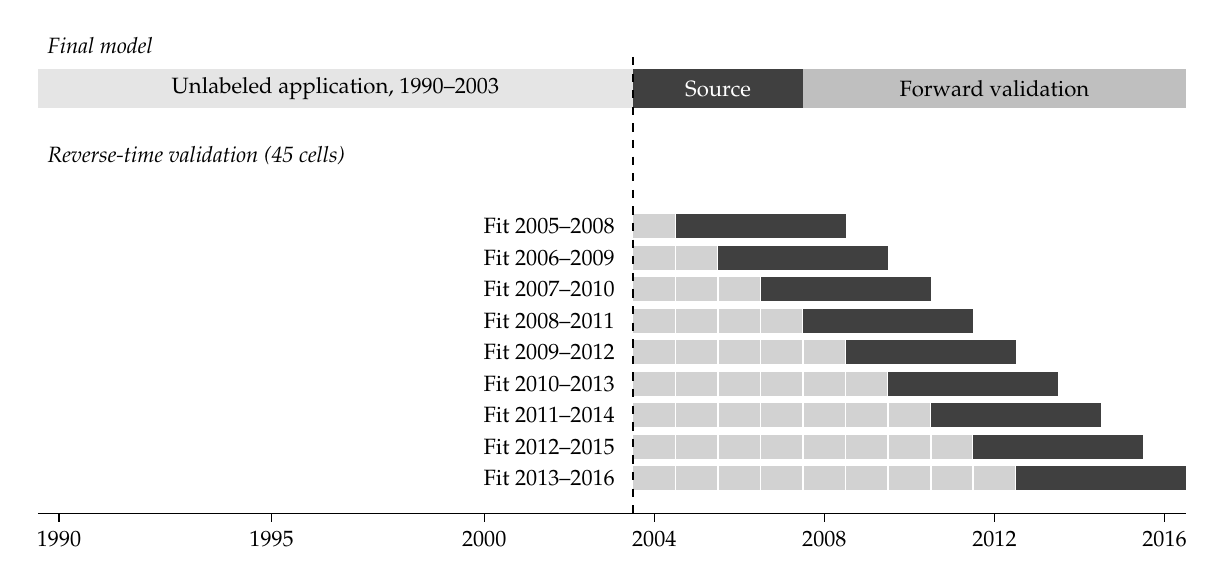
\begin{tikzpicture}[x=0.54cm, y=0.5cm, font=\footnotesize]
		% Final design: application, source, and forward validation.
		\node[anchor=west, font=\footnotesize\itshape] at (0, 1.6) {Final model};
		\fill[gray!20] (0, 0) rectangle (14, 1);
		\fill[black!75] (14, 0) rectangle (18, 1);
		\fill[gray!50] (18, 0) rectangle (27, 1);
		\node at (7, 0.5) {Unlabeled application, 1990--2003};
		\node[text=white] at (16, 0.5) {Source};
		\node at (22.5, 0.5) {Forward validation};
		% Reverse-time validation triangle.
		\node[anchor=west, font=\footnotesize\itshape] at (0, -1.2)
			{Reverse-time validation (45 cells)};
		\foreach \k in {1, ..., 9} {
			\pgfmathsetmacro{\ytop}{-1.9 - 0.8 * \k}
			\pgfmathsetmacro{\ybot}{\ytop - 0.6}
			\pgfmathtruncatemacro{\sy}{2004 + \k}
			\pgfmathtruncatemacro{\ey}{2007 + \k}
			\fill[gray!35] (14, \ybot) rectangle (\sy - 1990, \ytop);
			\foreach \t in {2005, ..., \sy} {
				\draw[white, line width=0.6pt] (\t - 1990, \ybot) -- (\t - 1990, \ytop);
			}
			\fill[black!75] (\sy - 1990, \ybot) rectangle (\sy - 1986, \ytop);
			\node[anchor=east] at (13.8, {(\ytop + \ybot) / 2}) {Fit \sy--\ey};
		}
		% Year axis.
		\draw (0, -10.3) -- (27, -10.3);
		\foreach \t in {1990, 1995, 2000, 2004, 2008, 2012, 2016} {
			\draw (\t - 1990 + 0.5, -10.3) -- (\t - 1990 + 0.5, -10.5);
			\node[anchor=north] at (\t - 1990 + 0.5, -10.5) {\t};
		}
		\draw[dashed] (14, 1.3) -- (14, -10.3);
	\end{tikzpicture}
	\caption{Data and Validation Timeline}
	\label{fig:timeline}
	\begin{figurenotes}
		Dark bars are four-year source windows; light gray cells in the lower panel are the
		labeled target years evaluated by each reverse-time fit. The dashed line marks the
		start of lien-status reporting in 2004. Horizon is the first source year minus the
		target year. The final model is fitted on 2004--2007, validated forward on 2008--2016,
		and applied backward to 1990--2003.
	\end{figurenotes}
	\todo{Move this figure to the introduction as Figure 1 once that section is drafted.}
\end{figure}

\subsection{Frozen challengers}\label{sec:est_challengers}

Four challengers, all fixed before the comparisons reported below, test how much the results
depend on functional form, the external county-value input, and model family.
Table~\ref{tab:protocol} summarizes them; Appendix~\ref{app:estimator} documents their
selection.
\begin{enumerate}
	\item \emph{Unrestricted gradient boosting.} A histogram gradient-boosted classifier
	\citep{friedman2001greedy,ke2017lightgbm}, as implemented in scikit-learn
	\citep{pedregosa2011scikit}, uses the four primitive predictors, with purchaser and loan
	type as native categorical variables. It has no splines or hand-built interactions. The
	selected configuration has seven leaves per tree, a learning rate of 0.05, 200 iterations,
	an L2 penalty of 1, and at least 1,000 loans per leaf.
	\item \emph{HMDA-only logistic.} The HMDA-only logistic model uses the $\log(\text{LTI})$
	spline and the purchaser- and loan-type indicators without interactions, with $C = 1$. It
	was selected from the analogous grid restricted to HMDA predictors.
	\item \emph{HMDA-only boosting.} This model drops $x_2$ from the boosting model. Its
	independent search selected the same hyperparameters as the unrestricted model.
	\item \emph{Fixed Random Forest.} A random forest \citep{breiman2001random} with 50 trees of
	maximum depth 10 uses the untransformed continuous predictors and full categorical
	indicators. This is the configuration of the original exploratory classifier, and it is not
	tuned further. It serves as an appendix robustness benchmark.
\end{enumerate}

The family-specific selection objectives differed. The logistic specification was selected on
raw-probability Brier score, while boosting was selected on mixture-adjusted Brier. For the
comparisons in this paper, each finalist is therefore refit under one common convention: equal
source-year class weights \eqref{eq:weights}, fitted log odds interpreted as the log density
ratio (tree-based probabilities are clipped to $[10^{-12}, 1 - 10^{-12}]$ before taking log
odds), the annual mixture adjustment \eqref{eq:mixture_likelihood}--\eqref{eq:adjusted_probability},
identical target observations, and identical metrics. This convention changes how the fitted
models are scored but does not reopen either search.

The families differ most in how they extrapolate. Because the logistic spline has linear tails
and the county-value ratio enters linearly, the logistic model extends the log density ratio
linearly outside the source support. A tree ensemble instead holds its prediction constant
beyond its outermost split, carrying terminal-leaf values into regions it never observed. This
distinction matters because the historical covariate distribution differs materially from its
2004--2007 counterpart.

\begin{table}[htbp]
	\centering
	\caption{Estimators and Validation Protocol}
	\label{tab:protocol}
	\small
	\inputpaper{table2_estimator_protocol.tex}

	\vspace{1ex}
	\begin{tablenotes}
		One row per finalist: predictor set, functional form, fixed hyperparameters, source
		years, source weighting, target adjustment, and role in the paper. Every finalist is
		fitted with equal first- and second-lien mass within each source year and receives the
		same annual mixture-share adjustment. Reverse validation uses nine four-year windows
		and 45 cells. Forward validation fits on 2004--2007 and evaluates 2008--2016.
	\end{tablenotes}
	\todo{Generate from the persisted artifact metadata sidecars and frozen protocol
	constants.}
\end{table}

\fi

\begin{spacing}{1}
  {\small
    \bibliographystyle{jpe}
	\bibliography{\drop/bib/master,hmda}
  }
\end{spacing}

\clearpage
\appendix
\renewcommand\thefigure{\thesection.\arabic{figure}}
\renewcommand\thetable{\thesection.\arabic{table}}
\setcounter{figure}{0}
\setcounter{table}{0}

\ifclaude
[CLAUDE]

\section{Data Construction and County-Value Scaling}\label{app:data}

\subsection{Sample attrition}

Table~\ref{tab:app_attrition} reports cumulative sample attrition for every year. The stages
are applied in the order listed in Section~\ref{sec:data_sample}. Pooled over 1990--2016, the
counts before the county-value merge are 542,378,694 raw records; 95,451,637 originated,
owner-occupied, home-purchase loans; 92,429,861 with a valid state and county; 90,232,646 with
positive, nonmissing income and loan amount; and 90,232,611 with a standard loan type. In labeled
years, the lien-status requirement removes no loans from this population.
\todo{Add the pooled post-merge and final common-sample totals once the audit is regenerated
with the year-specific county-value panel; the pre-merge stages above are unchanged.}

\begin{table}[htbp]
	\centering
	\caption{Annual Sample Attrition}
	\label{tab:app_attrition}
	\small
	\inputpaper{tableA1_attrition_by_year.tex}

	\vspace{1ex}
	\begin{tablenotes}
		Cumulative counts after each restriction. ``Common model sample'' additionally
		requires finite values of all four predictors, so every model scores the same loans.
		Source: \texttt{output/tables/sample\_attrition\_by\_year.csv}.
	\end{tablenotes}
\end{table}

\subsection{County-value scaling}

\paragraph{Why the native FHFA level cannot be used.} The FHFA county workbook normalizes each
county's index to 100 in the county's first observed year, so its cross-county level depends on
when the series began rather than on relative house prices. Among counties observed throughout
1990--2016, the ratio of the native index to a common-1990-base index ranges from 0.51 to 5.56,
and the cross-county correlation between the native and common-base indexes is only 0.06 in
2000. A common base removes the arbitrary normalization but still produces an appreciation
index rather than a price level. The exploratory classifier that preceded this paper used the
native-index ratio, and we replace it with the Zillow-scaled value in \eqref{eq:county_value}.

\paragraph{Scale estimator and alternatives.} The primary scale is the geometric-mean
Zillow-to-FHFA ratio over all overlap years. We also compute three alternatives: least squares
in levels through the origin, $Z_{ct} = a_c H_{ct} + e_{ct}$; the median annual log ratio; and
the single-year 2017 ratio. Across the 2,690 primary counties, the levels estimator is nearly
identical to the primary one: the median absolute log difference is 0.0009 and the 99th
percentile is 0.022. The median-ratio estimator has a median difference of zero and a 99th
percentile of 0.043. The single-year anchor is less stable, with a median log difference of
0.032 and a 90th percentile of 0.118, which supports multi-year pooling. The within-county root
mean squared log residual of the geometric fit has a median of 0.041 and a 90th percentile of
0.092. These residuals reflect conceptual and dynamic differences between the two indexes, so
$\widehat{V}_{ct}$ should not be read as an estimate of an individual property's value.

\paragraph{Overlap support.} Of the 2,690 scaled counties, 249 have exactly one overlap year
and 29 have two. Requiring three overlap years would retain 2,412 counties.
\todo{Report the three-overlap-year support robustness check if it is run.}

\paragraph{Year-specific versus balanced county panels.} An earlier version of the sample
required each county to have an FHFA observation in every year from 1990 through 2016. That
balanced panel contains only 1,431 counties and matches 95.1 percent of otherwise eligible
loans, compared with more than 99 percent for year-specific matching in most years. More
importantly, it is correlated with lien status: in 2004--2007 it retains 93.8--95.1 percent of
first liens but 97.4--98.0 percent of second liens, raising the observed second-lien share by
0.35--0.56 percentage point. The year-specific merge raises the source-period share by only
0.03 percentage point. It changes the county composition over time, however, so
Table~\ref{tab:app_coverage} reports annual loan and county coverage.

\begin{table}[htbp]
	\centering
	\caption{County-Value Coverage}
	\label{tab:app_coverage}
	\small
	\inputpaper{tableA2_county_value_coverage.tex}

	\vspace{1ex}
	\begin{tablenotes}
		Share of otherwise eligible loans and reported county codes matched to a scaled
		county value, by year, and match rates by observed lien status in 2004--2016. Sources:
		\texttt{output/tables/county\_value\_coverage\_by\_year.csv} and
		\texttt{county\_value\_coverage\_by\_lien\_status.csv}.
	\end{tablenotes}
\end{table}

\subsection{Source harmonization and missing features}

Annual LAR files come from several distributors, whose layouts and variable names differ. A
versioned loader maps each provider's native names and types to one canonical schema, and the
resolved source is recorded with each cleaned annual extract. Categorical predictors are
encoded against fixed canonical levels (all ten purchaser-type codes and all four loan types).
The design matrix therefore has identical columns in every year, even when a level is absent.
The only missing-feature exclusions are the loans with missing purchaser type in 1990, 1991,
and 1999 reported in Section~\ref{sec:data_sample}.
\todo{Add a source-by-year table and the purchaser-type crosswalk discussion.}

\section{Estimator Details and Model Selection}\label{app:estimator}

\subsection{Logistic feature matrix}

\paragraph{Spline basis.} Given knots $k_1 < k_2 < k_3 < k_4$ at the 5th, 35th, 65th, and 95th
source percentiles of $x_1$, the restricted cubic spline has the linear term $x_1$ and, for
$j = 1, 2$,
\begin{equation}
	h_j(x_1) = \frac{(x_1 - k_j)_+^3
		- \frac{k_4 - k_j}{k_4 - k_3} (x_1 - k_3)_+^3
		+ \frac{k_3 - k_j}{k_4 - k_3} (x_1 - k_4)_+^3}{(k_4 - k_1)^2} ,
\end{equation}
where $(u)_+ = \max(u, 0)$. The basis is cubic between knots, and its second derivative vanishes
beyond $k_4$ and below $k_1$, so the fitted function is linear in both tails
\citep{harrell2015regression}. Each of the three basis columns is centered and scaled by its
source-window mean and standard deviation. The linear county-value term and the continuous
parts of the purchaser interactions use standardized $x_1$ and $x_2$. The interactions are
linear in $x_1$ even though the $x_1$ main effect is a spline.

\paragraph{Column structure.} The 34 slope columns consist of three spline terms for $x_1$, one
linear term for $x_2$, nine purchaser-type indicators, three loan-type indicators, nine
$x_1$-by-purchaser interactions, and nine $x_2$-by-purchaser interactions. The reference levels
are purchaser type 0 (not sold within the calendar year) and conventional loans.
Table~\ref{tab:app_logit_spec} reports the fitted knots, standardization constants, and
coefficients of the final 2004--2007 known-source-prior model.

\paragraph{Estimation.} We solve \eqref{eq:ridge} with a Newton--Cholesky solver, a convergence
tolerance of $10^{-8}$, and an iteration limit of 200. Nonconverged fits would be rerun with a
larger limit rather than compared as though early stopping were a model choice.
\todo{Confirm that every selection-grid fit converged at the default limit.}

\begin{table}[htbp]
	\centering
	\caption{Final Logistic Specification}
	\label{tab:app_logit_spec}
	\small
	\inputpaper{tableB1_logistic_specification.tex}

	\vspace{1ex}
	\begin{tablenotes}
		Feature names, reference levels, spline knots (on the $\log(\text{LTI})$ scale),
		standardization constants, and estimated coefficients of the 2004--2007
		equal-source-prior ridge logistic model ($C = 0.1$). The same constants are distributed
		with the portable prediction package.
	\end{tablenotes}
\end{table}

\subsection{Weighting, mixture likelihood, and adjusted probabilities}

\paragraph{Weighted source population.} Under \eqref{eq:weights}, the total weight of class $y$
in year $s$ is $N_s/2$. Normalizing by the total weight $N_{\mathcal{W}} = \sum_s N_s$, the
reweighted source population has $\Pr^w(y = 1) = 1/2$ and class-conditional density $\bar{f}_y
= \sum_s (N_s / N_{\mathcal{W}}) f_s(\cdot \mid y)$. The weighted log likelihood in
\eqref{eq:ridge} is the sample analogue of the expected log likelihood in this population, and
its population minimizer, absent the penalty and under correct specification, satisfies
\eqref{eq:density_ratio}. Because the equal-class weights are applied within each source year,
year-to-year changes in source prevalence do not enter the intercept.

\paragraph{Mixture likelihood.} Write $\hat{r}_i = \hat{r}(x_i)$ and $D_i(\pi) = 1 - \pi +
\pi \hat{r}_i$. Then $\ell_t'(\pi) = \sum_i (\hat{r}_i - 1)/D_i(\pi)$. Because $\tilde{p}_i(\pi)
- \pi = \pi (1 - \pi)(\hat{r}_i - 1)/D_i(\pi)$,
\begin{equation}
	\sum_{i} \pbrac{\tilde{p}_i(\pi) - \pi} = \pi (1 - \pi)\, \ell_t'(\pi) ,
\end{equation}
so any interior stationary point satisfies \eqref{eq:fixed_point}. The EM update $\pi \leftarrow
N_t^{-1} \sum_i \tilde{p}_i(\pi)$ has the same fixed point. We maximize $\ell_t$ over $[10^{-9},
1 - 10^{-9}]$, compute all terms in log space, and flag estimates within ten times the bound of
either endpoint. We then run EM from the optimizer's solution as a consistency check.
\todo{Report the maximum optimizer-versus-EM difference and boundary counts, which appear in
the validation findings (below $6 \times 10^{-9}$, with no boundary estimates in any design).}

\paragraph{Intercept representation.} By \eqref{eq:adjusted_probability}, the adjusted
probability in year $t$ is a logistic model with the fitted slope coefficients and intercept
$\hat{\alpha} + \operatorname{logit} \hat{\pi}_t$. The released portable predictor stores the
slope coefficients once, together with this annual intercept for every year from 1990 through
2016. Applying it to a subset of loans reproduces the full-sample adjusted probabilities; it
does not re-estimate a subset-specific share.

\paragraph{Normalization moments.} A valid density ratio satisfies $\E_0[r(X)] = 1$ and
$\E_1[1/r(X)] = 1$. The equal-prior logistic fit matches weighted score equations instead, and
in the reverse source folds both empirical moments depart substantially from one. The departure
for $\E_0[\hat{r}]$ is driven by a small mass of very large fitted ratios: in target years, the
log ratio has a median near $-4.5$, a 99th percentile near 6.3, and a 99.9th percentile near
10.8. These tails do not prevent the share likelihood from converging to an interior optimum in
any validation or historical year, but they rule out a literal structural reading of $\hat{r}$.
\todo{Replace with exact moment ranges from output/tables/mixture\_ratio\_fit\_diagnostics.csv.}

\subsection{Logistic model selection}

\paragraph{Unrestricted grid.} Every candidate includes both continuous predictors and both
sets of categorical indicators. The frozen grid crosses three continuous forms (linear; a spline
in $x_1$ only; splines in both) with four interaction structures (none; continuous-by-loan-type;
continuous-by-purchaser-type; both), for twelve specifications. Interactions are linear slope
deviations, and there are no continuous-by-continuous terms. The penalty is searched over $C
\in \{10^{-4}, 10^{-2}, 1, 100\}$, followed by the two adjacent decades around each
specification's best coarse value, with outward extension if the winner lies on the boundary.
The selection statistic is the raw-probability Brier score, unweighted and without prevalence
adjustment, aggregated by \eqref{eq:horizon_average} over the 45 reverse cells. The selected
pair is the $x_1$ spline with purchaser-type interactions and $C = 0.1$.

\paragraph{Post-selection challengers.} Three predeclared challengers were evaluated against the
selected core without automatic replacement. First, interacting every $x_1$ spline-basis term
with purchaser type also selects $C = 0.1$ but worsens equal-horizon Brier and is worse at every
horizon from 2 through 9, so it is rejected. Second, adding Census-region indicators lowers
Brier in 44 of 45 cells. We do not adopt it, because broad geographic effects estimated in the
2000s may proxy for period-specific market structure when transported to the early 1990s.
Third, adding state indicators does not improve the equal-horizon score.
\todo{Decide whether to report the region challenger's historical series as an additional
robustness check. Report the results of the mixture-native coordinate search around the
incumbent, if completed.}

\paragraph{HMDA-only grid.} The restricted grid crosses a linear or spline $x_1$ with the same
four interaction structures, for eight specifications. It uses the same penalty search and
objective, on the same sample. It selects the $x_1$ spline without interactions and $C = 1$.

\begin{table}[htbp]
	\centering
	\caption{Logistic Selection Summary}
	\label{tab:app_logit_selection}
	\small
	\inputpaper{tableB2_logistic_selection.tex}

	\vspace{1ex}
	\begin{tablenotes}
		Equal-horizon raw Brier score for the best penalty of each specification in the
		unrestricted and HMDA-only grids, with the selected pair marked. Sources:
		\texttt{logistic\_selection\_core\_\{coarse,refinement\}\_summary.csv} and
		\texttt{logistic\_selection\_decision.csv}.
	\end{tablenotes}
\end{table}

\subsection{Gradient-boosting selection}

The boosting search uses scikit-learn's histogram gradient-boosting classifier with binary log
loss, equal source-prior weights, 255 bins, a minimum of 1,000 loans per leaf, a fixed random
seed, and no internal early-stopping split. Iteration count is instead an explicit candidate. The
search has three predeclared stages. (i) On the latest source window, 2013--2016, which is
evaluated at every horizon from 1 to 9, it screens trees with 7, 15, or 31 leaves and learning
rates of 0.05 or 0.1, holding 200 iterations and an L2 penalty of 1. (ii) The two structures with
the lowest equal-horizon mixture-adjusted Brier are evaluated on all 45 cells. (iii) Around the
better survivor, four one-dimensional refinements set the iterations to 100 or 400 or the L2
penalty to 0 or 10. The selection statistic is mixture-adjusted Brier aggregated by
\eqref{eq:horizon_average}. The unrestricted and HMDA-only searches, run separately,
select the same configuration: seven leaves, a learning rate of 0.05, 200 iterations, and an L2
penalty of 1. The search is deliberately bounded, and it is not intended to exhaust the boosting
parameter space.

\begin{table}[htbp]
	\centering
	\caption{Gradient-Boosting Selection Summary}
	\label{tab:app_boost_selection}
	\small
	\inputpaper{tableB3_boosting_selection.tex}

	\vspace{1ex}
	\begin{tablenotes}
		Screen, survivor, and refinement candidates with their equal-horizon mixture-adjusted
		Brier scores, for the unrestricted and HMDA-only predictor sets. Sources: the
		boosting screen, survivor, refinement, and decision tables.
	\end{tablenotes}
\end{table}

\subsection{Random Forest robustness model}

The Random Forest keeps the exploratory classifier's settings: 50 trees, a maximum depth of 10,
and a fixed seed. It uses the two untransformed continuous predictors and full one-hot encodings
of purchaser and loan type, with no splines, interactions, or additional variables. It is
fitted with the equal source-prior weights and no additional class weighting, and it receives
the same mixture adjustment as the other finalists. No forest hyperparameter was chosen using
validation results.

\subsection{Artifacts and reproducibility}

Every fitted model---each reverse-window fit, each candidate in each selection stage, and each
final 2004--2007 fit---is saved together with a metadata record. The record contains the schema
version, a SHA-256 digest of the serialized model, the model and configuration identity, the
source years, the training counts by class, the feature schema, the weighting and source-prior
convention, and the software versions. Grid and historical jobs publish immutable result shards,
and aggregation refuses missing, duplicate, or conflicting shards. Only fitted parameters and
aggregate diagnostics are retained. Loan-level probabilities and target-year characteristics
are computed in memory and never written to disk. The unrestricted and HMDA-only logistic models,
including their annual intercepts for 1990--2016, are distributed as a dependency-light
prediction package. On synthetic inputs spanning every category combination, the spline
knots, and both tails, it reproduces the original fitted probabilities to within $10^{-12}$.
\todo{Add repository URL and package version.}

\fi

\end{document}
